\documentclass[UTF8,11pt,a4paper]{ctexart}

% ---------- 页面设置 ----------
\usepackage[top=2.2cm, bottom=2.2cm, left=2.2cm, right=2.2cm]{geometry}
\usepackage{amsmath,amssymb,amsfonts}
\usepackage{graphicx}
\usepackage{booktabs,multirow,array}
\usepackage[colorlinks=true,linkcolor=black,citecolor=black]{hyperref}
\usepackage{caption}
\usepackage{setspace}
\usepackage{indentfirst}
\usepackage{abstract}
\usepackage{float}
\usepackage{enumitem}
\usepackage{listings}
\usepackage{xcolor}
\lstset{
    language=Python,
    basicstyle=\small\ttfamily,
    numbers=left,
    numberstyle=\tiny\color{gray},
    stepnumber=1,
    frame=single,
    breaklines=true,
    showstringspaces=false,
    commentstyle=\color{teal},
    keywordstyle=\color{blue},
    stringstyle=\color{red!80!black},
    extendedchars=true,
    numbersep=5pt,
    xleftmargin=15pt,
    framexleftmargin=15pt,
}

% 行距与段落
\setstretch{1.0}
\setlength{\parskip}{0.3em}

% 节标题格式
\ctexset{section/format={\large\bfseries}}
\ctexset{subsection/format={\normalsize\bfseries}}

% 图/表编号
\captionsetup{labelsep=space, font=small}

\begin{document}

% ============================================================
% 标题
% ============================================================
\title{\vspace{-2em}\textbf{AI 技术采纳对企业劳动生产率的因果效应}\\\textbf{——基于双重机器学习的实证分析}}
\author{}
\date{}
\maketitle
\vspace{-3em}

% ============================================================
% 摘要
% ============================================================
\begin{abstract}
\noindent 人工智能技术的快速发展引发了关于其对企业生产率影响的广泛讨论。本文基于 Global AI Adoption \& Workforce Impact 数据集（150{,}000 家企业观测，2023--2026 年），采用双重机器学习（Double/Debiased Machine Learning, DML）方法，在部分线性模型框架下估计 AI 技术采纳对企业劳动生产率的因果效应。通过 Neyman 正交评分与交叉拟合技术，DML 允许在控制高维协变量的同时实现稳健的推断。实证结果表明，在控制行业、规模、自动化率、创新能力等企业特征后，AI 采纳对劳动生产率的因果效应为 0.006，在统计上不显著（$p = 0.342$）。该结论在随机森林、LASSO、XGBoost 三种机器学习方法以及不同的交叉拟合折数（$K = 2,5,10$）下均保持稳健。进一步分析显示，仅将全面采纳（full adoption）定义为处理组时效应显著为正（$\hat\theta = 0.056$, $p = 0.030$），但该结果需谨慎解读。研究表明，AI 采纳与企业生产率之间的正向关联很大程度上可由企业特征差异所解释，而非直接的因果效应。
\end{abstract}

% ============================================================
% 1. 引言
% ============================================================
\section{引言}\label{sec:intro}

人工智能（AI）作为一项通用技术，正深刻重塑全球产业格局。企业对 AI 技术的采纳是否切实提升了生产率，是经济学界和实务界共同关注的焦点问题。现有研究对此尚未形成一致结论：一方面，部分研究发现 AI 显著提升了企业绩效~\cite{acemoglu2018race}；另一方面，AI 的生产率效应可能存在滞后性，且在不同行业和企业间呈现显著异质性~\cite{bresnahan2002information}。

从计量经济学角度看，识别 AI 采纳对生产率的因果效应面临两重挑战：一是\textbf{混淆因素}——采纳 AI 的企业往往在规模、创新能力、数字化水平等方面与未采纳企业存在系统性差异，这些差异同时影响采纳决策和生产率；二是\textbf{高维控制}——潜在的混淆因素数量多、形式复杂（包括非线性关系和高阶交互效应），传统的参数回归方法难以灵活控制。

双重机器学习（Double/Debiased Machine Learning, DML）由 Chernozhukov 等~\cite{chernozhukov2018double} 提出，为解决上述挑战提供了有效框架。DML 在部分线性模型下利用机器学习方法灵活估计高维非线性 nuisance 函数，并通过 Neyman 正交评分和交叉拟合保证因果参数的 $\sqrt{N}$-一致估计和渐近正态推断。

本文基于 Kaggle 平台 Global AI Adoption \& Workforce Impact 数据集（150{,}000 条企业观测），采用 DML 方法估计 AI 技术采纳对企业劳动生产率的因果效应。研究结果表明：（1）在控制企业特征后，AI 采纳（部分采纳或全面采纳）对劳动生产率的因果效应不显著（$\hat\theta = 0.006$, $p = 0.342$）；（2）该结论在多种设定下保持稳健；（3）仅全面采纳 AI 的企业表现出显著的生产率提升（$\hat\theta = 0.056$, $p = 0.030$），但处理组仅占样本的 1.1\%。本文的结构如下：第~\ref{sec:data} 节介绍数据来源与描述性统计；第~\ref{sec:model} 节建立部分线性模型并阐述 DML 估计方法；第~\ref{sec:results} 节报告实证结果与稳健性检验；第~\ref{sec:conclusion} 节总结全文。

% ============================================================
% 2. 数据
% ============================================================
\section{数据}\label{sec:data}

\subsection{数据来源}

本文使用的数据来自 Kaggle 平台发布的 Global AI Adoption \& Workforce Impact Dataset\footnote{https://www.kaggle.com/datasets/mohankrishnathalla/global-ai-adoption-and-workforce-impact-dataset}。该数据集包含 2023 年至 2026 年全球 30 个国家 9 个行业共 150{,}000 条企业级观测，记录了企业的 AI 采纳阶段、财务状况、劳动力结构、运营特征以及治理实践等多维度信息，无缺失值。

\subsection{变量设计与选择理由}

\textbf{处理变量 $D$：AI 采纳程度。}数据中的 AI 采纳阶段包含四个类别：无采纳（none, 3.5\%）、试验阶段（pilot, 42.9\%）、部分采纳（partial, 52.5\%）和全面采纳（full, 1.1\%）。本文将部分采纳和全面采纳定义为高采纳组（$D = 1$），其余为低采纳组（$D = 0$），得到 53.7\% 的处理组与 46.3\% 的对照组，分组均衡。

\textbf{结果变量 $Y$：劳动生产率。}参照 Syverson~\cite{syverson2011determinants} 的标准做法，以人均营收的对数衡量：$Y = \log(\text{Annual Revenue} / \text{Employees})$。

\textbf{协变量 $X$：企业特征。}为控制混淆因素，选取以下维度的协变量：基本特征（行业、国家、地区、规模、年龄）、时间固定效应（年份、季度）、运营特征（自动化率、远程办公比例）、治理与创新（监管合规评分、数据隐私水平、AI 伦理委员会、风险管理评分、创新评分、员工满意度）。通过 one-hot 编码后协变量总维度为 64。

\subsection{描述性统计}

\begin{table}[H]
\centering
\caption{主要变量描述性统计}
\label{tab:descriptive}
\small
\setlength{\tabcolsep}{4pt}
\begin{tabular}{lcccc}
\toprule
变量 & 均值 & 标准差 & 最小值 & 最大值 \\
\midrule
劳动生产率（对数） & $-0.747$ & 0.935 & $-4.428$ & 2.247 \\
AI 高采纳（$D=1$） & 0.537 & 0.499 & 0 & 1 \\
企业年龄 & 18.507 & 9.539 & 1.000 & 36.000 \\
自动化率（\%） & 19.762 & 9.223 & 0.000 & 59.630 \\
创新评分 & 55.200 & 8.593 & 40.000 & 97.000 \\
员工满意度 & 5.601 & 0.815 & 2.100 & 9.200 \\
监管合规评分 & 70.398 & 9.406 & 40.000 & 100.000 \\
AI 风险管理评分 & 59.566 & 8.851 & 40.000 & 98.000 \\
远程办公比例（\%） & 43.191 & 14.363 & 0.000 & 100.000 \\
员工数 & 2342.377 & 4754.425 & 10.000 & 19970.000 \\
营收（百万美元） & 1180.346 & 2391.471 & 1.010 & 9996.730 \\
\bottomrule
\multicolumn{5}{l}{\footnotesize 注：样本量 $N = 150{,}000$，数据不含缺失值。}
\end{tabular}
\end{table}

\begin{figure}[H]
\centering
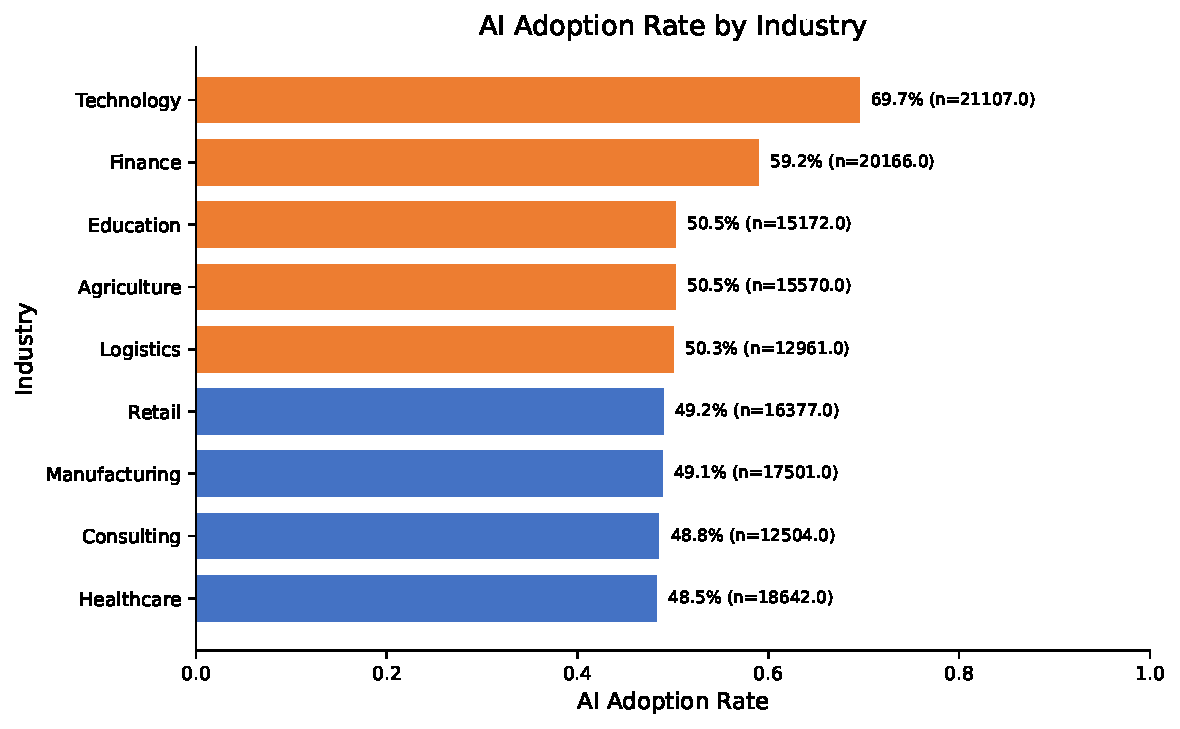
\includegraphics[width=0.47\textwidth]{../output/figures/fig1_ai_adoption_by_industry.pdf}
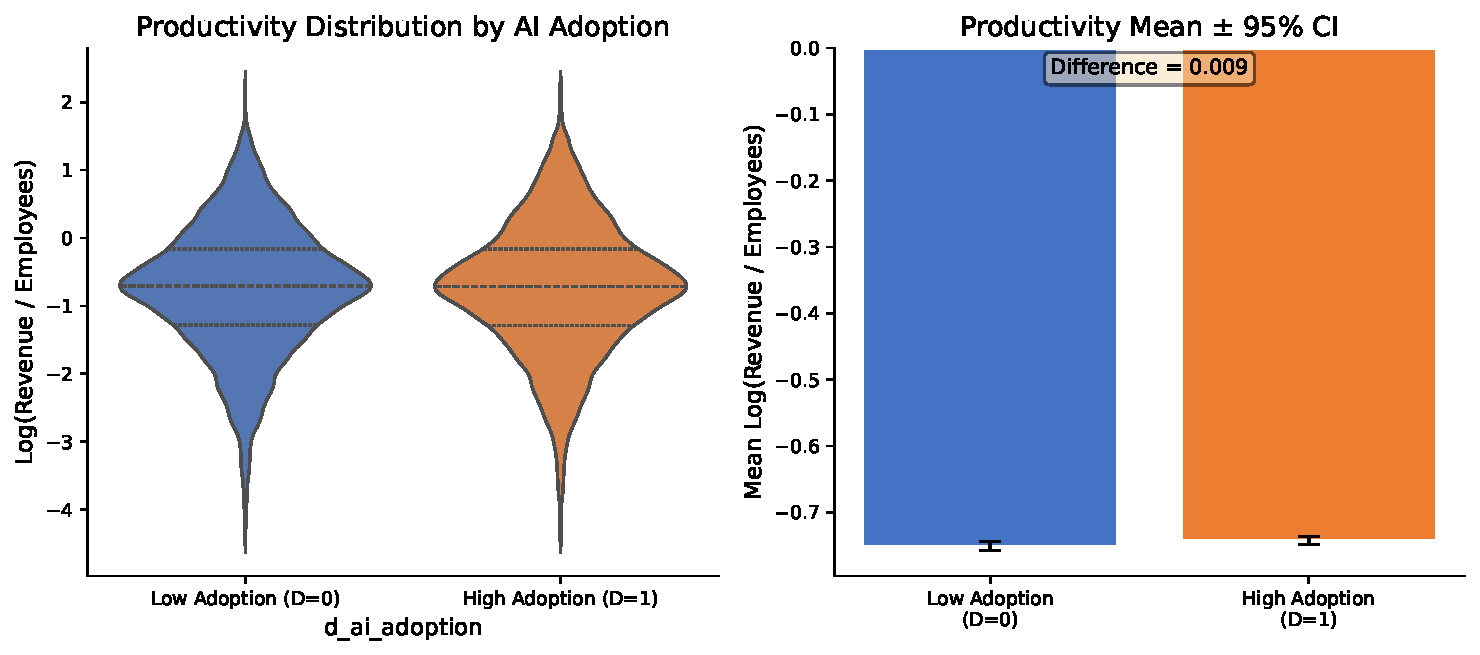
\includegraphics[width=0.47\textwidth]{../output/figures/fig2_productivity_by_adoption.pdf}
\caption{左：各行业 AI 采纳率（展示行业异质性）；右：不同采纳状态下的劳动生产率分布对比}
\label{fig:eda}
\end{figure}

表~\ref{tab:descriptive} 报告了主要变量的描述性统计。样本覆盖初创企业（37.8\%）、中小企业（42.6\%）和大型企业（19.6\%），行业涵盖科技（14.1\%）、金融（13.4\%）、医疗（12.4\%）等九个领域。图~\ref{fig:eda} 展示了数据的基本特征：左图显示行业间 AI 采纳率差异较大（约 40\%--70\%），表明行业是重要混淆因素；右图显示高采纳组与低采纳组的劳动生产率分布十分接近，原始差异很小（均值差仅为 0.009），这为后续因果分析提供了初步线索。

% ============================================================
% 3. 模型建立
% ============================================================
\section{模型建立}\label{sec:model}

\subsection{部分线性模型}

本文采用部分线性模型（Partial Linear Model）刻画 AI 采纳与劳动生产率之间的关系：
\begin{align}
Y_i &= \theta_0 D_i + g_0(X_i) + \varepsilon_i, \quad \mathbb{E}[\varepsilon_i \mid X_i, D_i] = 0, \label{eq:plm_y} \\
D_i &= m_0(X_i) + \nu_i, \quad \mathbb{E}[\nu_i \mid X_i] = 0. \label{eq:plm_d}
\end{align}
其中 $Y_i$ 为劳动生产率的对数，$D_i$ 为 AI 采纳的二元处理变量，$X_i$ 为高维协变量向量。参数 $\theta_0$ 是核心待估参数——AI 采纳的平均处理效应（ATE）。函数 $g_0(\cdot)$ 和 $m_0(\cdot)$ 为未知的 nuisance 函数，由机器学习方法灵活估计。该模型将因果参数 $\theta_0$ 与 nuisance 函数分离，为 DML 方法的应用提供了基础框架。

\subsection{DML 估计量}

DML 方法基于 Neyman 正交评分函数构造估计量。对部分线性模型，评分函数为：
\begin{equation}\label{eq:score}
\psi(W; \theta, \eta) = \bigl(Y - \ell(X) - \theta \bigl(D - m(X)\bigr)\bigr) \bigl(D - m(X)\bigr),
\end{equation}
其中 $\ell(X) = \mathbb{E}[Y \mid X]$，$m(X) = \mathbb{E}[D \mid X]$。该评分满足 Neyman 正交性：$\partial \mathbb{E}[\psi(W; \theta_0, \eta_0)] / \partial \eta = 0$，即 nuisance 参数的估计误差对 $\theta_0$ 的影响是二阶小量。这一性质保证了即使使用灵活的机器学习方法估计 $\ell$ 和 $m$，$\theta$ 的估计仍能达到 $\sqrt{N}$-收敛率。

给定 nuisance 函数的估计 $\hat\ell$ 和 $\hat m$，DML 估计量求解 $\frac{1}{N}\sum_i \psi(W_i; \hat\theta, \hat\eta) = 0$，得到：
\begin{equation}\label{eq:dml_estimator}
\hat\theta = \frac{\sum_{i=1}^N \tilde D_i \tilde Y_i}{\sum_{i=1}^N \tilde D_i^2},
\end{equation}
其中 $\tilde Y_i = Y_i - \hat\ell(X_i)$，$\tilde D_i = D_i - \hat m(X_i)$ 为残差。直觉上，DML 先通过机器学习"剔除"协变量 $X$ 对 $Y$ 和 $D$ 的影响，再对剩余的变异进行 OLS 回归。

\subsection{交叉拟合}

若用全样本估计 nuisance 函数再在相同数据上估计 $\theta$，会因过拟合产生偏差。交叉拟合（cross-fitting）技术用于避免这一问题，具体流程如下：

\begin{enumerate}[leftmargin=*,nosep]
\item 将样本随机等分为 $K$ 折（本文取 $K = 5$）。
\item 对每折 $k = 1,\dots,K$：
  \begin{enumerate}[nosep]
    \item 在除第 $k$ 折外的所有样本上训练 $\hat\ell^{(-k)}$ 和 $\hat m^{(-k)}$。
    \item 在第 $k$ 折上计算残差 $\tilde Y_i = Y_i - \hat\ell^{(-k)}(X_i)$，$\tilde D_i = D_i - \hat m^{(-k)}(X_i)$。
  \end{enumerate}
\item 合并所有残差，代入式~\eqref{eq:dml_estimator} 得 $\hat\theta$。
\item 采用 Eicker--Huber--White 稳健标准误进行推断：
  \begin{equation*}
    \widehat{\mathrm{Var}}(\hat\theta) = \frac{\sum_i \tilde D_i^2 \hat\varepsilon_i^2}{\bigl(\sum_i \tilde D_i^2\bigr)^2}, \quad
    \hat\varepsilon_i = \tilde Y_i - \hat\theta \tilde D_i.
  \end{equation*}
\end{enumerate}

\subsection{机器学习方法}

基线设定使用\textbf{随机森林}（RF, $n_{\text{estimators}}=100$, $\max_{\text{depth}}=10$, $\min_{\text{samples leaf}}=10$），能自动捕捉非线性关系和交互效应。稳健性检验中进一步使用\textbf{LASSO}（交叉验证选择 $\lambda$）和\textbf{XGBoost}（$n_{\text{estimators}}=100$, $\max_{\text{depth}}=4$, 学习率 0.1）估计 nuisance 函数。

% ============================================================
% 4. 实证结果
% ============================================================
\section{实证结果}\label{sec:results}

\subsection{基准结果}

\begin{table}[H]
\centering
\caption{基准 DML 估计结果}
\label{tab:baseline}
\small
\begin{tabular}{lcccccc}
\toprule
方法 & ATE & 标准误 & 95\% 置信区间 & $p$ 值 & 样本量 \\
\midrule
DML（RF, $K=5$） & 0.0059 & 0.0062 & $[-0.0063,\;0.0180]$ & 0.342 & 150{,}000 \\
\midrule
原始均值差异 & 0.0088 & --- & --- & --- & 150{,}000 \\
\bottomrule
\end{tabular}
\end{table}

表~\ref{tab:baseline} 报告了基准 DML 估计结果。在控制行业、规模、自动化率、创新能力等企业特征后，AI 采纳的 ATE 为 0.0059（标准误 0.0062，$p = 0.342$），统计上不显著。点估计对应的劳动生产率为约 0.6\% 的提升，经济意义有限。作为参照，高采纳组与低采纳组的原始均值差异为 0.0088，与 DML 估计值在量级上接近——表明在控制可观测特征后，因果效应估计与原始差异方向一致但估计精度不足以拒绝零假设。

\textbf{讨论：}一个可能解释是数据集覆盖的企业多处于 AI 采纳的早期阶段（全面采纳仅占 1.1\%）。按 Nelson~\&~Phelps（1966）的技术扩散理论，企业需要一定的学习和调整时间才能将新技术转化为生产率增长。若数据采集时大部分企业刚进入采纳阶段，因果效应可能尚未充分显现。

\subsection{稳健性检验}

\begin{table}[H]
\centering
\caption{稳健性检验结果}
\label{tab:robustness}
\small
\setlength{\tabcolsep}{4pt}
\begin{tabular}{lcccl}
\toprule
设定 & ATE & 标准误 & 95\% CI & $p$ 值 \\
\midrule
\textbf{（1）更换 ML 方法} & & & & \\
\quad LASSO（CV） & 0.0004 & 0.0064 & $[-0.0121,\;0.0129]$ & 0.948 \\
\quad XGBoost & 0.0042 & 0.0065 & $[-0.0085,\;0.0168]$ & 0.519 \\
\midrule
\textbf{（2）改变折数} & & & & \\
\quad $K = 2$ & 0.0058 & 0.0063 & $[-0.0065,\;0.0181]$ & 0.354 \\
\quad $K = 10$ & 0.0051 & 0.0062 & $[-0.0070,\;0.0172]$ & 0.407 \\
\midrule
\textbf{（3）严格处理定义} & & & & \\
\quad 仅 full = 1 & 0.0557 & 0.0256 & $[0.0055,\;0.1060]$ & 0.030 \\
\midrule
\textbf{（4）替换结果变量} & & & & \\
\quad 生产率变化（\%） & 2.698 & 0.029 & $[2.640,\;2.756]$ & $<0.001$ \\
\bottomrule
\end{tabular}
\end{table}

表~\ref{tab:robustness} 汇总了四项稳健性检验的结果：

\textbf{（1）更换 ML 方法。}LASSO 和 XGBoost 的 ATE 分别为 0.0004（$p = 0.948$）和 0.0042（$p = 0.519$），与基线高度一致。三种差异巨大的机器学习方法得到一致结论，显著增强了结果的可信度。

\textbf{（2）改变交叉拟合折数。}$K = 2$ 和 $K = 10$ 的 ATE 分别为 0.0058 和 0.0051，几乎无异于基线。表明 DML 估计对样本分割方式不敏感。

\textbf{（3）严格处理定义。}仅将全面采纳定义为处理组时，ATE 升至 0.0557（$p = 0.030$），在 5\% 水平上显著。这一结果需谨慎解读：一方面可能表明只有深度的 AI 采纳才能带来生产率提升；另一方面处理组仅 1.1\%（$n = 1{,}685$），估计精度有限。

\textbf{（4）替换结果变量。}使用自我报告的生产率变化百分比时，估计值为 2.698（$p < 0.001$），高度显著。但该变量为回顾性主观评价，易受测量误差和反向因果影响。

综合来看，基准结果在多种设定下保持稳健：控制企业特征后，AI 采纳对生产率的因果效应不显著。

\subsection{内生性诊断}\label{sec:diagnostics}

本节通过四项检验评估 DML 识别假设的合理性。\textbf{共同支撑检验}显示两组倾向得分在 $[0.1, 0.9]$ 区间内有良好重叠，极端占比均低于 1\%（图~\ref{fig:diagnostics} 左）。\textbf{安慰剂检验}将 $Y$ 随机打乱后重新估计，5 次重复中假阳性率为 0\%（所有 $p > 0.05$），DML 估计量没有系统性偏误。\textbf{协变量平衡检验}显示残差化后 $|\text{corr}(\tilde D, X)|$ 均值从 0.233 降至 0.017，$\hat m(\cdot)$ 有效吸收了协变量对 $D$ 的解释力。\textbf{灵敏度分析}（图~\ref{fig:diagnostics} 右）表明即使添加与 $\tilde D$ 偏相关达 0.6 的未观测混淆变量，ATE 仍不显著（$p > 0.27$）。综合四项诊断，DML 的识别假设在本研究中具有合理性。

\begin{figure}[H]
\centering
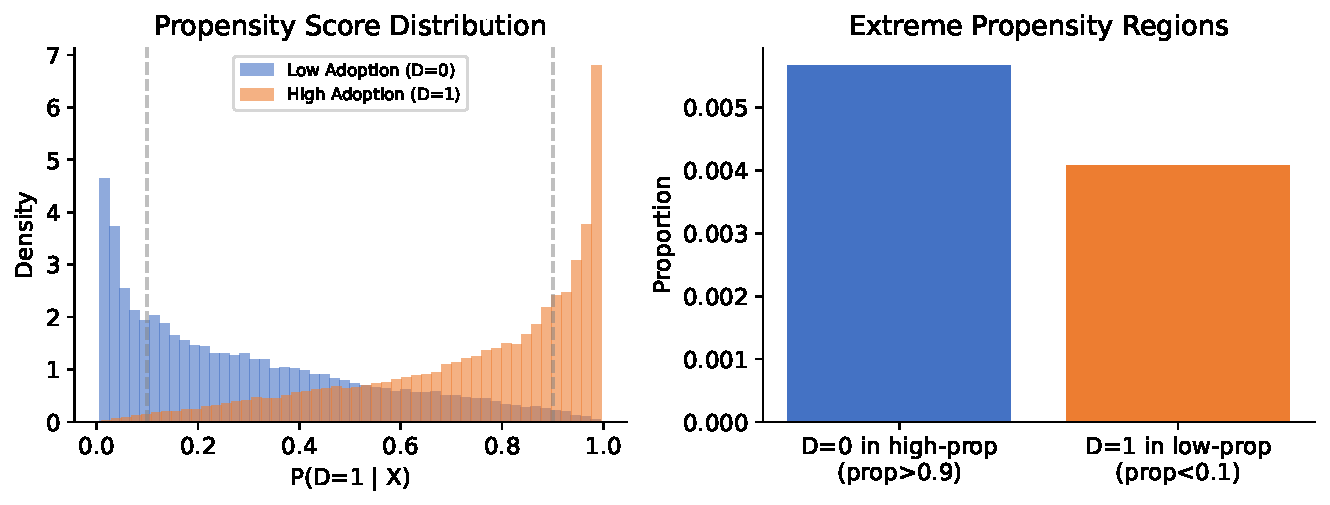
\includegraphics[width=0.47\textwidth]{../output/figures/fig5_overlap.pdf}
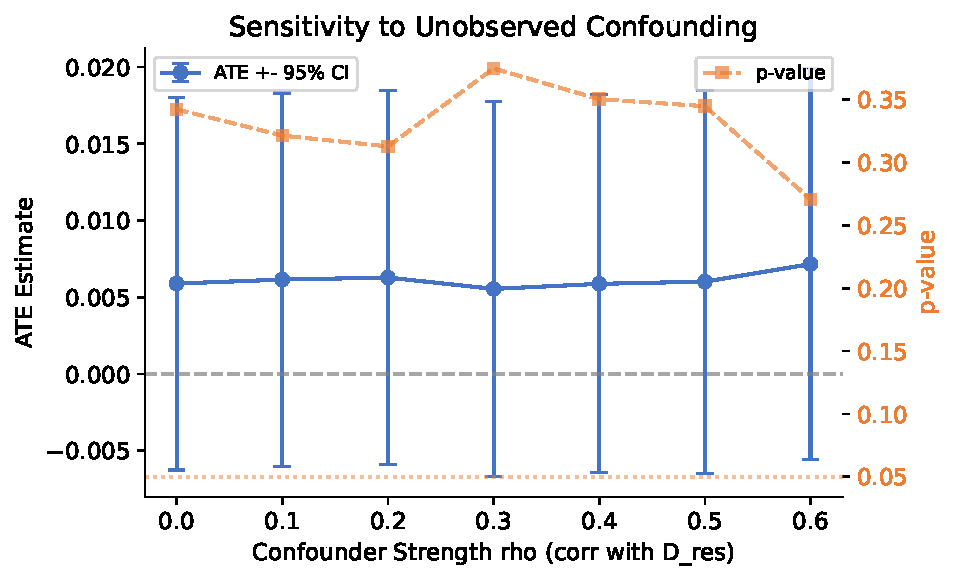
\includegraphics[width=0.47\textwidth]{../output/figures/fig7_sensitivity.pdf}
\caption{左：倾向得分分布（共同支撑）；右：未观测混淆灵敏度分析}
\label{fig:diagnostics}
\end{figure}

\subsection{异质性与多值处理}\label{sec:heterogeneity}

为进一步检验 AI 效应的异质性，本文分别在行业、企业规模、年份和自动化率四个维度进行子组 DML 估计，并以"无采纳"为参照组比较不同采纳深度的效应。

\begin{table}[H]
\centering
\caption{异质性分析结果}
\label{tab:heterogeneity}
\small
\setlength{\tabcolsep}{4pt}
\begin{tabular}{lcccc}
\toprule
子组 & ATE & SE & $p$ 值 & $N$ \\
\midrule
全样本（基准） & 0.006 & 0.006 & 0.342 & 150000 \\
大型企业 & 0.024 & 0.015 & 0.110 & 29448 \\
初创企业 & $-$0.007 & 0.011 & 0.518 & 56685 \\
零售 & 0.027 & 0.019 & 0.146 & 16377 \\
咨询 & $-$0.027 & 0.021 & 0.196 & 12504 \\
2026 年 & 0.016 & 0.013 & 0.221 & 37540 \\
Partial vs None & 0.031 & 0.026 & 0.234 & 83998 \\
\bottomrule
\end{tabular}
\end{table}

表~\ref{tab:heterogeneity} 报告了代表性子组的估计结果。所有子组的 ATE 均在统计上不显著（$p > 0.05$），进一步强化了"AI 采纳与生产率之间不存在显著因果效应"的核心结论。点估计呈现一些值得注意的模式：大型企业的效应（0.024）高于初创企业（$-$0.007），零售（0.027）高于咨询（$-$0.027），2026 年（0.016）高于 2023 年（0.004），部分采纳 vs 无采纳的效应（0.031）在三类多值比较中最高。这些方向性差异与经济直觉相符——大企业有更强的技术吸收能力、AI 效应可能需要时间积累——但均未达到统计显著水平，不宜过度解读。

% ============================================================
% 5. 结论
% ============================================================
\section{结论}\label{sec:conclusion}

本文采用双重机器学习方法，基于 Global AI Adoption \& Workforce Impact 数据集，实证研究了 AI 技术采纳对企业劳动生产率的因果效应。在使用三种机器学习方法控制高维协变量后，未发现 AI 采纳对劳动生产率有统计上显著的因果效应，点估计的经济意义也有限。该结论在多种稳健性检验下保持一致；异质性分析进一步表明，在行业、企业规模、年份和自动化率等子组中该效应均不显著。本文为 AI 生产率效应的实证文献提供了基于 DML 方法的新证据，揭示了 AI 采纳与生产率之间的原始关联很大程度上可由企业特征差异所解释。

本研究存在以下局限：一是数据为面板结构但本文仅进行了混合截面分析，未能利用企业固定效应控制不随时间变化的不可观测异质性；二是简单的二值化处理无法刻画 AI 采纳强度的渐进变化；三是 AI 的生产率效应可能存在滞后性。未来研究可在企业固定效应 DML、多值处理变量框架以及考虑滞后效应的动态设定等方向进行深入拓展。

% ============================================================
% 参考文献
% ============================================================
\begin{thebibliography}{9}
\small

\bibitem{acemoglu2018race}
D.~Acemoglu and P.~Restrepo.
\newblock The race between man and machine: Implications of technology for growth, factor shares, and employment.
\newblock \textit{American Economic Review}, 108(6):1488--1542, 2018.

\bibitem{bresnahan2002information}
T.~F.~Bresnahan, E.~Brynjolfsson, and L.~M.~Hitt.
\newblock Information technology, workplace organization, and the demand for skilled labor: Firm-level evidence.
\newblock \textit{Quarterly Journal of Economics}, 117(1):339--376, 2002.

\bibitem{chernozhukov2018double}
V.~Chernozhukov, D.~Chetverikov, M.~Demirer, E.~Duflo, C.~Hansen, W.~Newey, and J.~Robins.
\newblock Double/debiased machine learning for treatment and structural parameters.
\newblock \textit{The Econometrics Journal}, 21(1):C1--C68, 2018.

\bibitem{syverson2011determinants}
C.~Syverson.
\newblock What determines productivity?
\newblock \textit{Journal of Economic Literature}, 49(2):326--365, 2011.

\end{thebibliography}

\clearpage
\appendix
% ============================================================
% 附录：Python 代码
% ============================================================
\section{代码附录}\label{sec:appendix}

\subsection{数据预处理 (\texttt{01\_data\_prep.py})}

\begin{lstlisting}[language=Python]
import pandas as pd, numpy as np, os

PROJECT_ROOT = os.path.dirname(os.path.dirname(os.path.abspath(__file__)))
DATA_RAW_DIR = os.path.join(PROJECT_ROOT, "data", "raw")
OUTPUT_TABLES = os.path.join(PROJECT_ROOT, "output", "tables")
os.makedirs(OUTPUT_TABLES, exist_ok=True)
np.random.seed(42)

df = pd.read_csv(os.path.join(DATA_RAW_DIR, "ai_company_adoption.csv"))
# Normalize column names to lowercase underscore
col_rename = {}
for col in df.columns:
    norm = col.lower().strip().replace(" ", "_").replace("-", "_")
    norm = norm.replace("(", "").replace(")", "")
    col_rename[col] = norm
df = df.rename(columns=col_rename)

D_COL = "ai_adoption_stage"
Y_REVENUE = "annual_revenue_usd_millions"
Y_EMPLOYEES = "num_employees"
ID_COLS = ["response_id", "company_id"]

CAT_COVARIATES = [
    "industry", "country", "region", "company_size",
    "survey_year", "quarter", "company_age_group",
    "data_privacy_level", "ai_ethics_committee",
    "survey_source", "data_collection_method"
]

# D = 1 for partial/full adoption, 0 for none/pilot
HIGH_STAGES = ["partial", "full"]
df["d_ai_adoption"] = df[D_COL].apply(lambda x: 1 if str(x).lower() in HIGH_STAGES else 0)

# Y = log(revenue / employees)
df["y_log_productivity"] = np.log(df[Y_REVENUE] / df[Y_EMPLOYEES])

# Identify numeric covariates automatically
all_numeric = df.select_dtypes(include=[np.number]).columns.tolist()
NUM_COVARIATES = [c for c in all_numeric if c not in set(ID_COLS + [Y_REVENUE, Y_EMPLOYEES])]

# Save cleaned data
save_cols = list(dict.fromkeys(
    ["d_ai_adoption", "y_log_productivity", D_COL, Y_REVENUE, Y_EMPLOYEES]
    + [c for c in CAT_COVARIATES if c in df.columns]
    + NUM_COVARIATES
))
df[save_cols].to_csv(os.path.join(OUTPUT_TABLES, "cleaned_data.csv"), index=False)
\end{lstlisting}

\subsection{可视化 (\texttt{02\_visualization.py})}

\begin{lstlisting}[language=Python]
import pandas as pd, numpy as np, matplotlib.pyplot as plt, seaborn as sns, os
import warnings; warnings.filterwarnings("ignore")

PROJECT_ROOT = os.path.dirname(os.path.dirname(os.path.abspath(__file__)))
OUTPUT_TABLES = os.path.join(PROJECT_ROOT, "output", "tables")
OUTPUT_FIGURES = os.path.join(PROJECT_ROOT, "output", "figures")
os.makedirs(OUTPUT_FIGURES, exist_ok=True)

plt.rcParams.update({"figure.dpi": 150, "font.size": 11,
    "axes.spines.top": False, "axes.spines.right": False})
COLOR = ["#4472C4", "#ED7D31"]

df = pd.read_csv(os.path.join(OUTPUT_TABLES, "cleaned_data.csv"))

# Fig 1: AI adoption rate by industry
industry_rate = df.groupby("industry")["d_ai_adoption"].mean().sort_values()
fig, ax = plt.subplots(figsize=(8, 5))
colors = [COLOR[0] if v < 0.5 else COLOR[1] for v in industry_rate.values]
ax.barh(industry_rate.index, industry_rate.values, color=colors, edgecolor="white")
ax.set_xlabel("AI Adoption Rate"); ax.set_title("AI Adoption Rate by Industry")
for i, (idx, v) in enumerate(industry_rate.items()):
    ax.text(v + 0.01, i, f"{v:.1%}", va="center", fontsize=8)
plt.tight_layout()
fig.savefig(os.path.join(OUTPUT_FIGURES, "fig1_ai_adoption_by_industry.pdf"), bbox_inches="tight")
plt.close()

# Fig 2: Productivity distribution by adoption status
fig, axes = plt.subplots(1, 2, figsize=(10, 4.5))
sns.violinplot(data=df, x="d_ai_adoption", y="y_log_productivity",
               palette=[COLOR[0], COLOR[1]], inner="quartile", ax=axes[0])
axes[0].set_xticklabels(["Low Adoption (D=0)", "High Adoption (D=1)"])
axes[0].set_ylabel("Log(Revenue / Employees)"); axes[0].set_title("Productivity Distribution")

means = df.groupby("d_ai_adoption")["y_log_productivity"].agg(["mean", "sem"])
axes[1].bar([0, 1], means["mean"], yerr=1.96 * means["sem"],
            color=[COLOR[0], COLOR[1]], capsize=5, edgecolor="white")
axes[1].set_xticks([0, 1]); axes[1].set_xticklabels(["Low (D=0)", "High (D=1)"])
axes[1].set_ylabel("Mean Log Productivity"); axes[1].set_title("Mean $\pm$ 95% CI")
diff = means.loc[1, "mean"] - means.loc[0, "mean"]
axes[1].annotate(f"Diff = {diff:.3f}", xy=(0.5, 0.95), xycoords="axes fraction",
                 ha="center", bbox=dict(boxstyle="round", facecolor="wheat", alpha=0.5))
plt.tight_layout()
fig.savefig(os.path.join(OUTPUT_FIGURES, "fig2_productivity_by_adoption.pdf"), bbox_inches="tight")
plt.close()

# Fig 3: AI adoption by firm size
size_order = [s for s in ["Startup", "SME", "Enterprise"] if s in df["company_size"].unique()]
size_order += [s for s in df["company_size"].unique() if s not in size_order]
ct = pd.crosstab(df["company_size"], df["d_ai_adoption"], normalize="index")
ct = ct.reindex([s for s in size_order if s in ct.index])
fig, ax = plt.subplots(figsize=(7, 4.5))
ct.plot(kind="bar", stacked=True, ax=ax, color=[COLOR[0], COLOR[1]], edgecolor="white")
ax.set_ylabel("Proportion"); ax.set_title("AI Adoption by Company Size")
for i, size in enumerate(ct.index):
    ax.text(i, ct.loc[size, 1] / 2, f"{ct.loc[size, 1]:.0%}", ha="center",
            va="center", fontsize=10, color="white", fontweight="bold")
plt.tight_layout()
fig.savefig(os.path.join(OUTPUT_FIGURES, "fig3_adoption_by_firm_size.pdf"), bbox_inches="tight")
plt.close()

# Fig 4: Correlation heatmap
key_vars = [c for c in ["y_log_productivity", "d_ai_adoption", "ai_adoption_rate",
    "task_automation_rate", "ai_maturity_score", "innovation_score",
    "num_ai_tools_used", "employee_satisfaction_score", "regulatory_compliance_score"]
    if c in df.columns]
corr = df[key_vars].corr()
fig, ax = plt.subplots(figsize=(9, 7))
mask = np.triu(np.ones_like(corr, dtype=bool), k=1)
sns.heatmap(corr, mask=mask, annot=True, fmt=".2f", cmap="RdBu_r",
            center=0, square=True, linewidths=0.5, ax=ax)
ax.set_title("Correlation Matrix of Key Variables")
plt.tight_layout()
fig.savefig(os.path.join(OUTPUT_FIGURES, "fig4_correlation_heatmap.pdf"), bbox_inches="tight")
plt.close()
\end{lstlisting}

\subsection{核心 DML 估计 (\texttt{03\_dml\_estimation.py})}

\begin{lstlisting}[language=Python]
import pandas as pd, numpy as np, os, warnings, time
from sklearn.model_selection import KFold
from scipy import stats
from sklearn.ensemble import RandomForestRegressor
warnings.filterwarnings("ignore")

PROJECT_ROOT = os.path.dirname(os.path.dirname(os.path.abspath(__file__)))
OUTPUT_TABLES = os.path.join(PROJECT_ROOT, "output", "tables")
os.makedirs(OUTPUT_TABLES, exist_ok=True)
np.random.seed(42)

df = pd.read_csv(os.path.join(OUTPUT_TABLES, "cleaned_data.csv"))
Y = df["y_log_productivity"].values
D = df["d_ai_adoption"].values

# Covariates: predetermined firm characteristics
COVARIATE_COLS = [
    "industry", "country", "region", "company_size",
    "company_age", "company_age_group", "company_founding_year",
    "survey_year", "quarter",
    "task_automation_rate", "remote_work_percentage",
    "regulatory_compliance_score", "data_privacy_level",
    "ai_ethics_committee", "ai_risk_management_score",
    "employee_satisfaction_score", "innovation_score",
]
COVARIATE_COLS = [c for c in COVARIATE_COLS if c in df.columns]

# One-hot encoding; survey_year as categorical fixed effect
FORCE_CATEGORICAL = ["survey_year"]
numeric_x = [c for c in COVARIATE_COLS if c in df.select_dtypes(include=[np.number]).columns]
categorical_x = [c for c in COVARIATE_COLS if c in df.select_dtypes(include=["object"]).columns]
categorical_x = list(set(categorical_x + FORCE_CATEGORICAL))
numeric_x = [c for c in numeric_x if c not in categorical_x]
df_x = pd.get_dummies(df[COVARIATE_COLS], columns=categorical_x, drop_first=True)
X = df_x.values.astype(np.float64)

def dml_cross_fit(Y, D, X, model_y, model_t, n_folds=5, seed=42):
    """DML with cross-fitting and Neyman orthogonal score"""
    kf = KFold(n_splits=n_folds, shuffle=True, random_state=seed)
    n = len(Y)
    Y_res, D_res = np.zeros(n), np.zeros(n)
    for train_idx, test_idx in kf.split(X):
        # Estimate nuisance functions on training fold, compute residuals on test fold
        model_y.fit(X[train_idx], Y[train_idx])
        model_t.fit(X[train_idx], D[train_idx])
        Y_res[test_idx] = Y[test_idx] - model_y.predict(X[test_idx])
        D_res[test_idx] = D[test_idx] - model_t.predict(X[test_idx])
    # OLS on residuals: tilde_Y = theta * tilde_D
    theta = np.nansum(D_res * Y_res) / (np.nansum(D_res ** 2) + 1e-10)
    # Eicker-Huber-White robust standard errors
    e = Y_res - theta * D_res
    se = np.sqrt(np.nansum(D_res ** 2 * e ** 2) / ((np.nansum(D_res ** 2) ** 2) + 1e-10))
    t_val = theta / se
    p_val = 2 * (1 - stats.norm.cdf(abs(t_val)))
    return theta, se, theta - 1.96 * se, theta + 1.96 * se, p_val

# Baseline: Random Forest with K=5
rf_y = RandomForestRegressor(n_estimators=100, max_depth=10, min_samples_leaf=10,
                              random_state=42, n_jobs=-1)
rf_t = RandomForestRegressor(n_estimators=100, max_depth=10, min_samples_leaf=10,
                              random_state=42, n_jobs=-1)
theta, se, ci_l, ci_u, p_val = dml_cross_fit(Y, D, X, rf_y, rf_t, n_folds=5)

results = pd.DataFrame([{"method": "DML (Random Forest)", "estimate": theta,
    "std_err": se, "ci_lower": ci_l, "ci_upper": ci_u, "p_value": p_val,
    "n": len(Y), "n_covariates": X.shape[1], "n_folds": 5}])
results.to_csv(os.path.join(OUTPUT_TABLES, "dml_results.csv"), index=False)
\end{lstlisting}

\subsection{稳健性检验 (\texttt{04\_robustness.py})}

\begin{lstlisting}[language=Python]
import pandas as pd, numpy as np, os, warnings, time
from sklearn.model_selection import KFold
from scipy import stats
from sklearn.ensemble import RandomForestRegressor
from sklearn.linear_model import LassoCV
import xgboost as xgb
warnings.filterwarnings("ignore")

PROJECT_ROOT = os.path.dirname(os.path.dirname(os.path.abspath(__file__)))
OUTPUT_TABLES = os.path.join(PROJECT_ROOT, "output", "tables")
np.random.seed(42)

df = pd.read_csv(os.path.join(OUTPUT_TABLES, "cleaned_data.csv"))

def dml_cross_fit(Y, D, X, model_y, model_t, n_folds=5, seed=42):
    kf = KFold(n_splits=n_folds, shuffle=True, random_state=seed)
    n = len(Y); Y_res, D_res = np.zeros(n), np.zeros(n)
    for tr, te in kf.split(X):
        model_y.fit(X[tr], Y[tr]); Y_res[te] = Y[te] - model_y.predict(X[te])
        model_t.fit(X[tr], D[tr]); D_res[te] = D[te] - model_t.predict(X[te])
    theta = np.nansum(D_res * Y_res) / np.nansum(D_res ** 2)
    e = Y_res - theta * D_res
    se = np.sqrt(np.nansum(D_res ** 2 * e ** 2) / (np.nansum(D_res ** 2) ** 2))
    t = theta / se
    return theta, se, theta - 1.96 * se, theta + 1.96 * se, 2 * (1 - stats.norm.cdf(abs(t)))

COVARIATE_COLS = ["industry", "country", "region", "company_size", "company_age",
    "company_age_group", "company_founding_year", "survey_year", "quarter",
    "task_automation_rate", "remote_work_percentage", "regulatory_compliance_score",
    "data_privacy_level", "ai_ethics_committee", "ai_risk_management_score",
    "employee_satisfaction_score", "innovation_score"]
COVARIATE_COLS = [c for c in COVARIATE_COLS if c in df.columns]

def prepare_X(df, extra_exclude=None):
    cols = [c for c in COVARIATE_COLS if c not in (extra_exclude or [])]
    cat = [c for c in cols if c in df.select_dtypes(include=["object"]).columns]
    cat = list(set(cat + ["survey_year"]))
    return pd.get_dummies(df[cols], columns=cat, drop_first=True).values.astype(np.float64)

X_base, Y_base, D_base = prepare_X(df), df["y_log_productivity"].values, df["d_ai_adoption"].values

results = []
# Baseline (loaded from saved results)
bl = pd.read_csv(os.path.join(OUTPUT_TABLES, "dml_results.csv"))
results.append({"specification": "Baseline (RF, K=5)", "estimate": bl["estimate"].values[0],
    "std_err": bl["std_err"].values[0], "ci_lower": bl["ci_lower"].values[0],
    "ci_upper": bl["ci_upper"].values[0], "p_value": bl["p_value"].values[0]})

# 1a: LASSO with cross-validation
ly = LassoCV(cv=5, random_state=42, max_iter=5000)
lt = LassoCV(cv=5, random_state=42, max_iter=5000)
th, se, cl, cu, pv = dml_cross_fit(Y_base, D_base, X_base, ly, lt)
results.append({"specification": "LASSO (CV)", "estimate": th, "std_err": se,
    "ci_lower": cl, "ci_upper": cu, "p_value": pv})

# 1b: XGBoost
xy = xgb.XGBRegressor(n_estimators=100, max_depth=4, lr=0.1, random_state=42, n_jobs=-1, verbosity=0)
xt = xgb.XGBRegressor(n_estimators=100, max_depth=4, lr=0.1, random_state=42, n_jobs=-1, verbosity=0)
th, se, cl, cu, pv = dml_cross_fit(Y_base, D_base, X_base, xy, xt)
results.append({"specification": "XGBoost", "estimate": th, "std_err": se,
    "ci_lower": cl, "ci_upper": cu, "p_value": pv})

# 2: Different numbers of folds K = 2, 10
for K in [2, 10]:
    rf = RandomForestRegressor(n_estimators=100, max_depth=10, min_samples_leaf=10, random_state=42, n_jobs=-1)
    th, se, cl, cu, pv = dml_cross_fit(Y_base, D_base, X_base, rf, rf, n_folds=K)
    results.append({"specification": f"K = {K}", "estimate": th, "std_err": se,
        "ci_lower": cl, "ci_upper": cu, "p_value": pv})

# 3: Strict treatment definition (full adoption only)
D_strict = (df["ai_adoption_stage"].str.lower() == "full").astype(int).values
rf = RandomForestRegressor(n_estimators=100, max_depth=10, min_samples_leaf=10, random_state=42, n_jobs=-1)
th, se, cl, cu, pv = dml_cross_fit(Y_base, D_strict, X_base, rf, rf)
results.append({"specification": "Strict D (full only)", "estimate": th, "std_err": se,
    "ci_lower": cl, "ci_upper": cu, "p_value": pv})

# 4: Alternative outcome variable
if "productivity_change_percent" in df.columns:
    Y_alt = df["productivity_change_percent"].values
    X_alt = prepare_X(df, extra_exclude=["productivity_change_percent"])
    rf = RandomForestRegressor(n_estimators=100, max_depth=10, min_samples_leaf=10, random_state=42, n_jobs=-1)
    th, se, cl, cu, pv = dml_cross_fit(Y_alt, D_base, X_alt, rf, rf)
    results.append({"specification": "Alt Y (productivity_change)", "estimate": th,
        "std_err": se, "ci_lower": cl, "ci_upper": cu, "p_value": pv})

pd.DataFrame(results).to_csv(os.path.join(OUTPUT_TABLES, "robustness_results.csv"), index=False)
\end{lstlisting}

\subsection{内生性诊断 (\texttt{05\_diagnostics.py})}

\begin{lstlisting}[language=Python]
import pandas as pd, numpy as np, os, warnings, time
from sklearn.model_selection import KFold
from scipy import stats
from sklearn.ensemble import RandomForestRegressor
import matplotlib.pyplot as plt
warnings.filterwarnings("ignore")

PROJECT_ROOT = os.path.dirname(os.path.dirname(os.path.abspath(__file__)))
OUTPUT_TABLES = os.path.join(PROJECT_ROOT, "output", "tables")
OUTPUT_FIGURES = os.path.join(PROJECT_ROOT, "output", "figures")
os.makedirs(OUTPUT_FIGURES, exist_ok=True); np.random.seed(42)
plt.rcParams.update({"figure.dpi": 150, "axes.spines.top": False, "axes.spines.right": False})
COLOR = ["#4472C4", "#ED7D31"]

df = pd.read_csv(os.path.join(OUTPUT_TABLES, "cleaned_data.csv"))
COVARIATE_COLS = ["industry", "country", "region", "company_size", "company_age",
    "company_age_group", "company_founding_year", "survey_year", "quarter",
    "task_automation_rate", "remote_work_percentage", "regulatory_compliance_score",
    "data_privacy_level", "ai_ethics_committee", "ai_risk_management_score",
    "employee_satisfaction_score", "innovation_score"]

def build_X(df, extra_exclude=None):
    cols = [c for c in COVARIATE_COLS if c not in (extra_exclude or [])]
    cat = [c for c in cols if c in df.select_dtypes(include=["object"]).columns]
    cat = list(set(cat + ["survey_year"]))
    return pd.get_dummies(df[cols], columns=cat, drop_first=True).values.astype(np.float64)

X, Y, D = build_X(df), df["y_log_productivity"].values, df["d_ai_adoption"].values

def dml_cross_fit(Y, D, X, my, mt, n_folds=5, seed=42):
    kf = KFold(n_splits=n_folds, shuffle=True, random_state=seed)
    n = len(Y); Yr, Dr = np.zeros(n), np.zeros(n)
    for tr, te in kf.split(X):
        my.fit(X[tr], Y[tr]); mt.fit(X[tr], D[tr])
        Yr[te] = Y[te] - my.predict(X[te]); Dr[te] = D[te] - mt.predict(X[te])
    th = np.nansum(Dr * Yr) / (np.nansum(Dr ** 2) + 1e-10)
    e = Yr - th * Dr
    se = np.sqrt(np.nansum(Dr ** 2 * e ** 2) / (np.nansum(Dr ** 2) ** 2 + 1e-10))
    pv = 2 * (1 - stats.norm.cdf(abs(th / (se + 1e-10))))
    return th, se, th - 1.96 * se, th + 1.96 * se, pv, Dr, Yr

# --- 1. Common support (overlap) ---
rf_prop = RandomForestRegressor(n_estimators=100, max_depth=8, min_samples_leaf=10, random_state=42, n_jobs=-1)
rf_prop.fit(X, D); propensity = rf_prop.predict(X)

fig, axes = plt.subplots(1, 2, figsize=(9, 3.5))
for dv, c, lb in [(0, COLOR[0], "Low (D=0)"), (1, COLOR[1], "High (D=1)")]:
    axes[0].hist(propensity[D == dv], bins=50, alpha=0.6, color=c, label=lb, density=True)
axes[0].axvline(0.1, ls="--", color="gray", alpha=0.5)
axes[0].axvline(0.9, ls="--", color="gray", alpha=0.5)
axes[0].set_xlabel("P(D=1|X)"); axes[0].set_ylabel("Density"); axes[0].legend()
extreme_0 = np.mean((D == 0) & (propensity > 0.9))
extreme_1 = np.mean((D == 1) & (propensity < 0.1))
axes[1].bar(["D=0, prop>0.9", "D=1, prop<0.1"], [extreme_0, extreme_1], color=COLOR)
axes[1].set_ylabel("Proportion")
plt.tight_layout()
fig.savefig(os.path.join(OUTPUT_FIGURES, "fig5_overlap.pdf"), bbox_inches="tight")
plt.close()

# --- 2. Placebo test (shuffle Y) ---
placebo_pvals = []
for i in range(5):
    Ys = np.random.permutation(Y)
    th, se, _, _, pv, _, _ = dml_cross_fit(Ys, D, X,
        RandomForestRegressor(50, 8, 15, random_state=42+i, n_jobs=-1),
        RandomForestRegressor(50, 8, 15, random_state=42+i, n_jobs=-1))
    placebo_pvals.append(pv)
fpr = np.mean(np.array(placebo_pvals) < 0.05)

# --- 3. Covariate balance ---
_, _, _, _, _, Dr, _ = dml_cross_fit(Y, D, X,
    RandomForestRegressor(100, 10, 10, random_state=42, n_jobs=-1),
    RandomForestRegressor(100, 10, 10, random_state=42, n_jobs=-1))
num_vars = df[COVARIATE_COLS].select_dtypes(include=[np.number]).columns.tolist()
bal = pd.DataFrame([(v, abs(np.corrcoef(D, df[v].values)[0,1]),
                       abs(np.corrcoef(Dr, df[v].values)[0,1])) for v in num_vars],
                   columns=["var", "raw", "resid"]).sort_values("raw", ascending=False)

fig, ax = plt.subplots(figsize=(7, 4))
ax.scatter(range(len(bal)), bal["raw"], color=COLOR[0], label="|corr(D,X)|", alpha=0.7)
ax.scatter(range(len(bal)), bal["resid"], color=COLOR[1], label="|corr(D_res,X)|", alpha=0.7, marker="D")
ax.axhline(0.1, color="gray", ls="--", alpha=0.5)
ax.set_xticks(range(len(bal))); ax.set_xticklabels(bal["var"], rotation=45, ha="right", fontsize=8)
ax.set_ylabel("|Correlation|"); ax.legend()
plt.tight_layout()
fig.savefig(os.path.join(OUTPUT_FIGURES, "fig6_covariate_balance.pdf"), bbox_inches="tight")
plt.close()

# --- 4. Sensitivity to unobserved confounding ---
sens = []
for rho in np.arange(0, 0.61, 0.1):
    U = rho * Dr + np.sqrt(1 - rho**2) * np.random.randn(len(Y))
    U = (U - U.mean()) / U.std()
    th, se, _, _, pv, _, _ = dml_cross_fit(Y, D, np.column_stack([X, U]),
        RandomForestRegressor(100, 10, 10, random_state=42, n_jobs=-1),
        RandomForestRegressor(100, 10, 10, random_state=42, n_jobs=-1))
    sens.append({"rho": rho, "est": th, "se": se, "p": pv})
sens_df = pd.DataFrame(sens)

fig, ax1 = plt.subplots(figsize=(6.5, 4))
ax1.errorbar(sens_df["rho"], sens_df["est"], yerr=1.96*sens_df["se"],
             fmt="-o", color=COLOR[0], capsize=4, label="ATE +/- 95% CI")
ax1.axhline(y=0, color="gray", ls="--", alpha=0.7)
ax1.set_xlabel("Confounder Strength $\\rho$"); ax1.set_ylabel("ATE"); ax1.legend(loc="upper left")
ax2 = ax1.twinx()
ax2.plot(sens_df["rho"], sens_df["p"], "s--", color=COLOR[1], markersize=5, alpha=0.7, label="p-value")
ax2.axhline(y=0.05, color=COLOR[1], ls=":", alpha=0.5)
ax2.set_ylabel("p-value", color=COLOR[1]); ax2.tick_params(axis="y", labelcolor=COLOR[1])
ax2.legend(loc="upper right")
plt.tight_layout()
fig.savefig(os.path.join(OUTPUT_FIGURES, "fig7_sensitivity.pdf"), bbox_inches="tight")
plt.close()

# Save results
pd.DataFrame([("Overlap", f"Extreme {extreme_0:.3f}/{extreme_1:.3f}"),
    ("Placebo", f"FPR {fpr:.1%}"), ("Balance", f"Mean |corr|={bal['resid'].mean():.3f}"),
    ("Sensitivity", "Critical rho>0.6")], columns=["test", "detail"]
).to_csv(os.path.join(OUTPUT_TABLES, "diagnostics_results.csv"), index=False)
sens_df.to_csv(os.path.join(OUTPUT_TABLES, "sensitivity_analysis.csv"), index=False)
\end{lstlisting}

\subsection{异质性分析 (\texttt{06\_heterogeneity\_analysis.py})}

\begin{lstlisting}[language=Python]
import pandas as pd, numpy as np, os, warnings
from sklearn.model_selection import KFold
from scipy import stats
from sklearn.ensemble import RandomForestRegressor
import matplotlib.pyplot as plt
from concurrent.futures import ThreadPoolExecutor, as_completed
warnings.filterwarnings("ignore")

PROJECT_ROOT = os.path.dirname(os.path.dirname(os.path.abspath(__file__)))
OUTPUT_TABLES = os.path.join(PROJECT_ROOT, "output", "tables")
OUTPUT_FIGURES = os.path.join(PROJECT_ROOT, "output", "figures")
os.makedirs(OUTPUT_FIGURES, exist_ok=True); np.random.seed(42)
plt.rcParams.update({"figure.dpi": 150, "axes.spines.top": False, "axes.spines.right": False})

df = pd.read_csv(os.path.join(OUTPUT_TABLES, "cleaned_data.csv"))
COVARIATE_COLS = ["industry", "country", "region", "company_size", "company_age",
    "company_age_group", "company_founding_year", "survey_year", "quarter",
    "task_automation_rate", "remote_work_percentage", "regulatory_compliance_score",
    "data_privacy_level", "ai_ethics_committee", "ai_risk_management_score",
    "employee_satisfaction_score", "innovation_score"]

cat_cols = [c for c in COVARIATE_COLS if c in df.select_dtypes(include=["object"]).columns]
if "survey_year" in COVARIATE_COLS and "survey_year" not in cat_cols:
    cat_cols.append("survey_year")
X_full = pd.get_dummies(df[COVARIATE_COLS], columns=cat_cols, drop_first=True).values.astype(np.float64)
X_COLS = pd.get_dummies(df[COVARIATE_COLS], columns=cat_cols, drop_first=True).columns.tolist()
Y, D = df["y_log_productivity"].values, df["d_ai_adoption"].values
stages = df["ai_adoption_stage"].values

def dml_cross_fit(Y, D, X, my, mt, n_folds=5, seed=42):
    if len(Y) < 200 or np.sum(D > 0.5) < 30 or np.sum(D < 0.5) < 30:
        return np.nan, np.nan, np.nan, np.nan, np.nan, None, None
    kf = KFold(n_splits=n_folds, shuffle=True, random_state=seed)
    n = len(Y); Yr, Dr = np.zeros(n), np.zeros(n)
    for tr, te in kf.split(X):
        try:
            my.fit(X[tr], Y[tr]); mt.fit(X[tr], D[tr])
            Yr[te] = Y[te] - my.predict(X[te]); Dr[te] = D[te] - mt.predict(X[te])
        except: return np.nan, np.nan, np.nan, np.nan, np.nan, None, None
    th = np.nansum(Dr * Yr) / (np.nansum(Dr ** 2) + 1e-10)
    se = np.sqrt(np.nansum(Dr ** 2 * (Yr - th * Dr) ** 2) / (np.nansum(Dr ** 2) ** 2 + 1e-10))
    pv = 2 * (1 - stats.norm.cdf(abs(th / (se + 1e-10))))
    return th, se, th - 1.96 * se, th + 1.96 * se, pv, Dr, Yr

def rf(seed): return RandomForestRegressor(80, 8, 15, random_state=seed, n_jobs=-1)

# --- 1. Multi-value treatment (vs. "none" as reference) ---
mv_results = []
for label, treat, ctrl in [("Pilot vs None", "pilot", "none"),
    ("Partial vs None", "partial", "none"), ("Full vs None", "full", "none")]:
    mask = (stages == treat) | (stages == ctrl)
    idx = np.where(mask)[0]; D_sub = (stages[idx] == treat).astype(float)
    nf = min(5, max(2, min(D_sub.sum(), (1-D_sub).sum()) // 100))
    th, se, _, _, pv, _, _ = dml_cross_fit(Y[idx], D_sub, X_full[idx], rf(42), rf(43), n_folds=nf)
    mv_results.append({"comparison": label, "ATE": th, "SE": se, "p_value": pv, "n": len(idx)})
pd.DataFrame(mv_results).to_csv(os.path.join(OUTPUT_TABLES, "multivalue_results.csv"), index=False)

# --- 2. Heterogeneous treatment effects by subgroup ---
def make_configs():
    cfg = []
    for ind in df["industry"].unique():
        cfg.append((X_COLS, "industry", ind, df["industry"].values == ind, True))
    for sz in df["company_size"].unique():
        cfg.append((X_COLS, "company_size", sz, df["company_size"].values == sz, True))
    for yr in sorted(df["survey_year"].unique()):
        cfg.append((X_COLS, "survey_year", str(yr), df["survey_year"].values == yr, True))
    med = df["task_automation_rate"].median()
    cfg.append((X_COLS, "automation", "high", df["task_automation_rate"].values >= med, False))
    cfg.append((X_COLS, "automation", "low", df["task_automation_rate"].values < med, False))
    return cfg

def run_hte(args):
    xcols, dim, lev, mask, do_exclude = args
    idx = np.where(mask)[0]
    exc = [xcols.index(c) for c in xcols if c.startswith(dim + "_")] if do_exclude else []
    Xs = np.delete(X_full[idx], exc, axis=1) if exc else X_full[idx]
    nt, nc = int(D[idx].sum()), int((1-D[idx]).sum())
    if nt < 50 or nc < 50:
        return {"dim": dim, "level": lev, "ATE": np.nan, "SE": np.nan, "p": np.nan, "n": len(idx)}
    nf = min(3, max(2, min(nt, nc) // 50))
    th, se, _, _, pv, _, _ = dml_cross_fit(Y[idx], D[idx], Xs, rf(42), rf(43), n_folds=nf)
    return {"dim": dim, "level": lev, "ATE": th, "SE": se, "p": pv, "n": len(idx)}

hte_res = []
with ThreadPoolExecutor(max_workers=3) as ex:
    for f in as_completed([ex.submit(run_hte, c) for c in make_configs()]):
        hte_res.append(f.result())
hte_df = pd.DataFrame(hte_res)
hte_df.to_csv(os.path.join(OUTPUT_TABLES, "hte_results.csv"), index=False)

# --- 3. Forest plot ---
plot_df = hte_df.dropna(subset=["ATE"]).copy()
if len(plot_df) > 0:
    plot_df["label"] = plot_df["dim"] + ": " + plot_df["level"]
    plot_df = plot_df.sort_values("ATE")
    fig, ax = plt.subplots(figsize=(8, max(4, len(plot_df) * 0.35)))
    for i, (_, r) in enumerate(plot_df.iterrows()):
        c = "#ED7D31" if r["p"] < 0.05 else "#4472C4"
        ax.errorbar(r["ATE"], i, xerr=1.96*r["SE"], fmt="o", color=c, capsize=4)
    ax.axvline(x=0, color="gray", ls="--", alpha=0.7)
    ax.set_yticks(range(len(plot_df)))
    ax.set_yticklabels(plot_df["label"], fontsize=9)
    ax.set_xlabel("ATE (95% CI)"); ax.set_title("Heterogeneous Treatment Effects")
    plt.tight_layout()
    fig.savefig(os.path.join(OUTPUT_FIGURES, "fig8_hte_forest.pdf"), bbox_inches="tight")
    plt.close()
\end{lstlisting}


\end{document}
